% intro

The Real-time Transport Protocol (RTP)~\cite{rfc3550} is designed for
multimedia telephony (voice-over-IP, video conferencing, telepresence
systems), multimedia streaming (video-on-demand, live streaming), and
multimedia broadcast. RTP's design is based on the fundamental principles of
\textit {application-layer framing} and \textit{integrated layer
processing}~\cite{clark:alf}, to this end, RTP provides the following
mechanisms: source and payload type identification, stream synchronization,
packet loss and re-ordering, media stream monitoring. RTP utilizes the RTP
Control Protocol (RTCP) to report the performance of the media stream.
Figure~\ref{fig:3:rtp:model} describes the features provided by RTP and RTCP.
The media sender transmits encoded media encapsulated in RTP, in addition it
also sends RTCP Sender Reports (SR) to facilitate playback synchronization of
different media streams (typically audio and video). The receiver maintains a
dejitter buffer to reorder media packets and play them out as per the timing
information encoded in the packet. If a packet missing the receiver attempts
to either recover the lost packet or conceal the error. Lastly, the receiving
endpoint reports rough or detailed statistics that enables the media sender to
adapt its media encoding rate, change to a better codec, or vary the amount of
forward error correction.

\begin{figure}[!h]
\centering{
  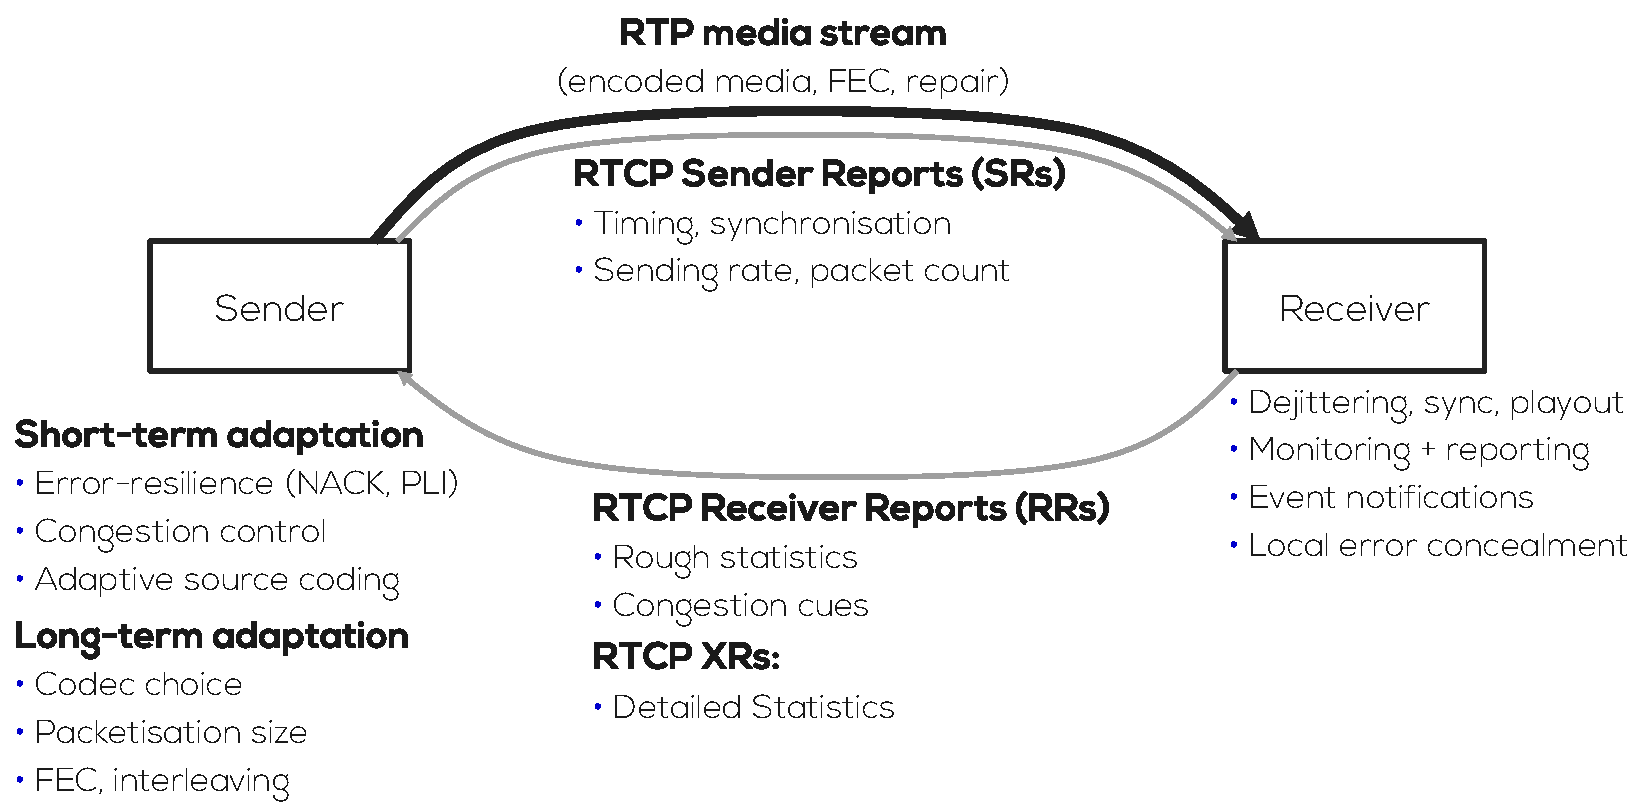
\includegraphics[width=\textwidth]{chap3-fig-rtp-rtcp}
}
\caption{RTP and RTCP for adaptive real-time applications {\scriptsize Source:
J\"org Ott, ``Networked Multimedia Protocols and Systems''}.}
\label{fig:3:rtp:model}
\end{figure}

Figure~\ref{fig:3:rtp.hdr} describes the RTP packet header format, the
\textit{`synchronization source'} (SSRC) assists in determining the source
endpoint, typically useful when an endpoint sends multiple media streams that
need to be synchronized (e.g., Audio/Video lip-sync). The \textit{`RTP
timestamp'} assists in playing out the received packets at the appropriate
instance of time and recomposing the media frame from RTP packets. The
\textit{`RTP sequence number'} assists in identifying the lost packets and re-
ordering packets in case of out-of-order packet arrival. Lastly, RTP uses
\textit{`payload type'} (PT) to describe the encoding of the media data it is
carrying. Consequently, each codec needs to specify its corresponding payload
format.

% \begin{figure}[!h]
% \centerline{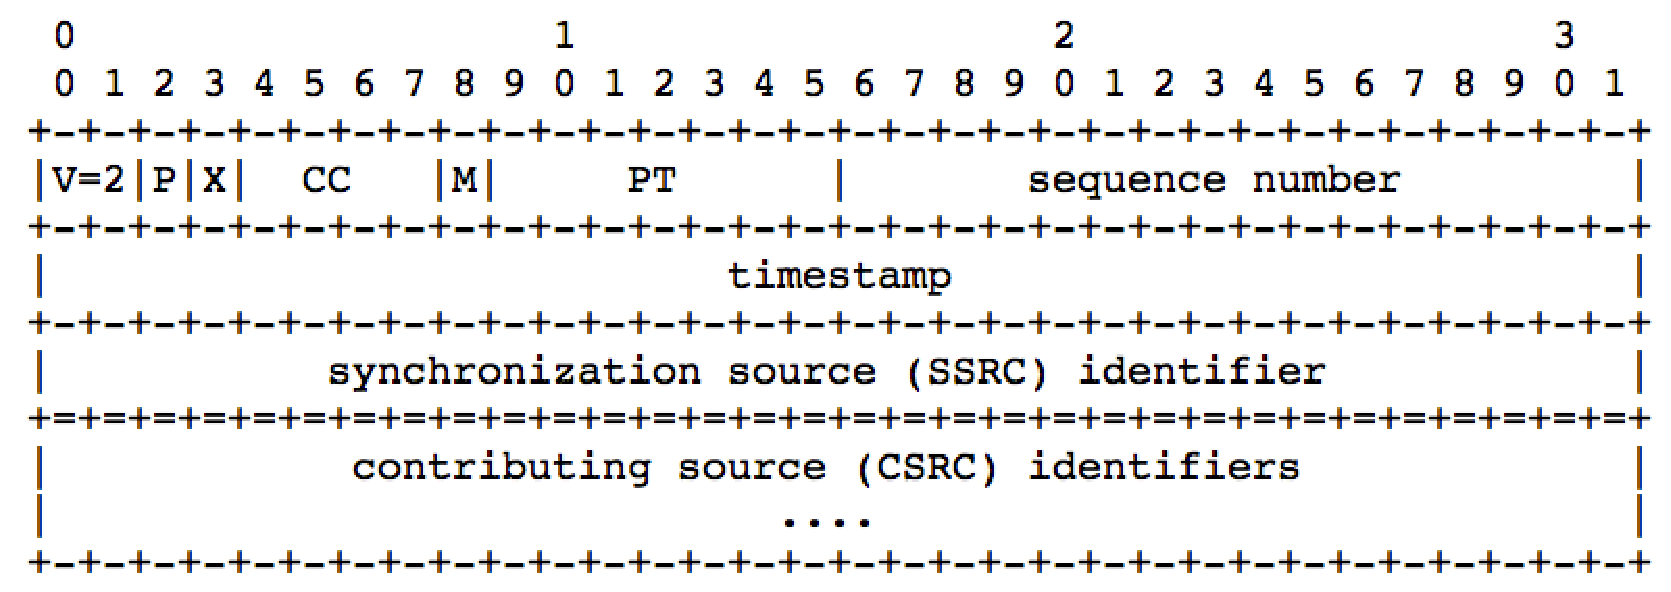
\includegraphics[width=\textwidth]{chap3_fig_hdr_rtp}}
% \caption{shows the RTP packet format that encapsulates the media data.}
% \label{fig:3:rtp.hdr}
% \end{figure}

\begin{figure}[!h]
\begin{spacing}{0.5}
\centering
{\small
\begin{verbatim}
    0                   1                   2                   3
    0 1 2 3 4 5 6 7 8 9 0 1 2 3 4 5 6 7 8 9 0 1 2 3 4 5 6 7 8 9 0 1
   +-+-+-+-+-+-+-+-+-+-+-+-+-+-+-+-+-+-+-+-+-+-+-+-+-+-+-+-+-+-+-+-+
   |V=2|P|X|  CC   |M|     PT      |       sequence number         |
   +-+-+-+-+-+-+-+-+-+-+-+-+-+-+-+-+-+-+-+-+-+-+-+-+-+-+-+-+-+-+-+-+
   |                           timestamp                           |
   +-+-+-+-+-+-+-+-+-+-+-+-+-+-+-+-+-+-+-+-+-+-+-+-+-+-+-+-+-+-+-+-+
   |           synchronization source (SSRC) identifier            |
   +=+=+=+=+=+=+=+=+=+=+=+=+=+=+=+=+=+=+=+=+=+=+=+=+=+=+=+=+=+=+=+=+
   |            contributing source (CSRC) identifiers             |
   |                             ....                              |
   +-+-+-+-+-+-+-+-+-+-+-+-+-+-+-+-+-+-+-+-+-+-+-+-+-+-+-+-+-+-+-+-+
\end{verbatim}
}
\end{spacing}
\caption{shows the RTP packet format that encapsulates the media data.}
\label{fig:3:rtp.hdr}
\end{figure}


\begin{figure}[!h]
\begin{spacing}{0.5}
{\footnotesize
\begin{verbatim}
          0                   1                   2                   3
          0 1 2 3 4 5 6 7 8 9 0 1 2 3 4 5 6 7 8 9 0 1 2 3 4 5 6 7 8 9 0 1
         +-+-+-+-+-+-+-+-+-+-+-+-+-+-+-+-+-+-+-+-+-+-+-+-+-+-+-+-+-+-+-+-+
  header |V=2|P|    RC   |   PT=SR=200   |             length            |
         +-+-+-+-+-+-+-+-+-+-+-+-+-+-+-+-+-+-+-+-+-+-+-+-+-+-+-+-+-+-+-+-+
         |                         SSRC of sender                        |
         +=+=+=+=+=+=+=+=+=+=+=+=+=+=+=+=+=+=+=+=+=+=+=+=+=+=+=+=+=+=+=+=+
  sender |              NTP timestamp, most significant word             |
  info   +-+-+-+-+-+-+-+-+-+-+-+-+-+-+-+-+-+-+-+-+-+-+-+-+-+-+-+-+-+-+-+-+
         |             NTP timestamp, least significant word             |
         +-+-+-+-+-+-+-+-+-+-+-+-+-+-+-+-+-+-+-+-+-+-+-+-+-+-+-+-+-+-+-+-+
         |                         RTP timestamp                         |
         +-+-+-+-+-+-+-+-+-+-+-+-+-+-+-+-+-+-+-+-+-+-+-+-+-+-+-+-+-+-+-+-+
         |                     sender's packet count                     |
         +-+-+-+-+-+-+-+-+-+-+-+-+-+-+-+-+-+-+-+-+-+-+-+-+-+-+-+-+-+-+-+-+
         |                      sender's octet count                     |
         +=+=+=+=+=+=+=+=+=+=+=+=+=+=+=+=+=+=+=+=+=+=+=+=+=+=+=+=+=+=+=+=+
  report |                 SSRC_1 (SSRC of first source)                 |
  block  +-+-+-+-+-+-+-+-+-+-+-+-+-+-+-+-+-+-+-+-+-+-+-+-+-+-+-+-+-+-+-+-+
    1    | fraction lost |       cumulative number of packets lost       |
         +-+-+-+-+-+-+-+-+-+-+-+-+-+-+-+-+-+-+-+-+-+-+-+-+-+-+-+-+-+-+-+-+
         |           extended highest sequence number received           |
         +-+-+-+-+-+-+-+-+-+-+-+-+-+-+-+-+-+-+-+-+-+-+-+-+-+-+-+-+-+-+-+-+
         |                      interarrival jitter                      |
         +-+-+-+-+-+-+-+-+-+-+-+-+-+-+-+-+-+-+-+-+-+-+-+-+-+-+-+-+-+-+-+-+
         |                         last SR (LSR)                         |
         +-+-+-+-+-+-+-+-+-+-+-+-+-+-+-+-+-+-+-+-+-+-+-+-+-+-+-+-+-+-+-+-+
         |                   delay since last SR (DLSR)                  |
         +=+=+=+=+=+=+=+=+=+=+=+=+=+=+=+=+=+=+=+=+=+=+=+=+=+=+=+=+=+=+=+=+
  report |                 SSRC_2 (SSRC of second source)                |
  block  +-+-+-+-+-+-+-+-+-+-+-+-+-+-+-+-+-+-+-+-+-+-+-+-+-+-+-+-+-+-+-+-+
    2    :                               ...                             :
         +=+=+=+=+=+=+=+=+=+=+=+=+=+=+=+=+=+=+=+=+=+=+=+=+=+=+=+=+=+=+=+=+
         |                  profile-specific extensions                  |
         +-+-+-+-+-+-+-+-+-+-+-+-+-+-+-+-+-+-+-+-+-+-+-+-+-+-+-+-+-+-+-+-+
\end{verbatim}
}
\end{spacing}
\caption{shows the RTCP packet format for carrying the Sender Report (SR) and
the Receiver Report (RR). The SR carries transport statistics and enables 
stream synchronization, while the RR carries the receiver transport 
characteristics.}
\label{fig:3:rtcp.hdr}
\end{figure}

% \begin{figure}[!h]
% \centering{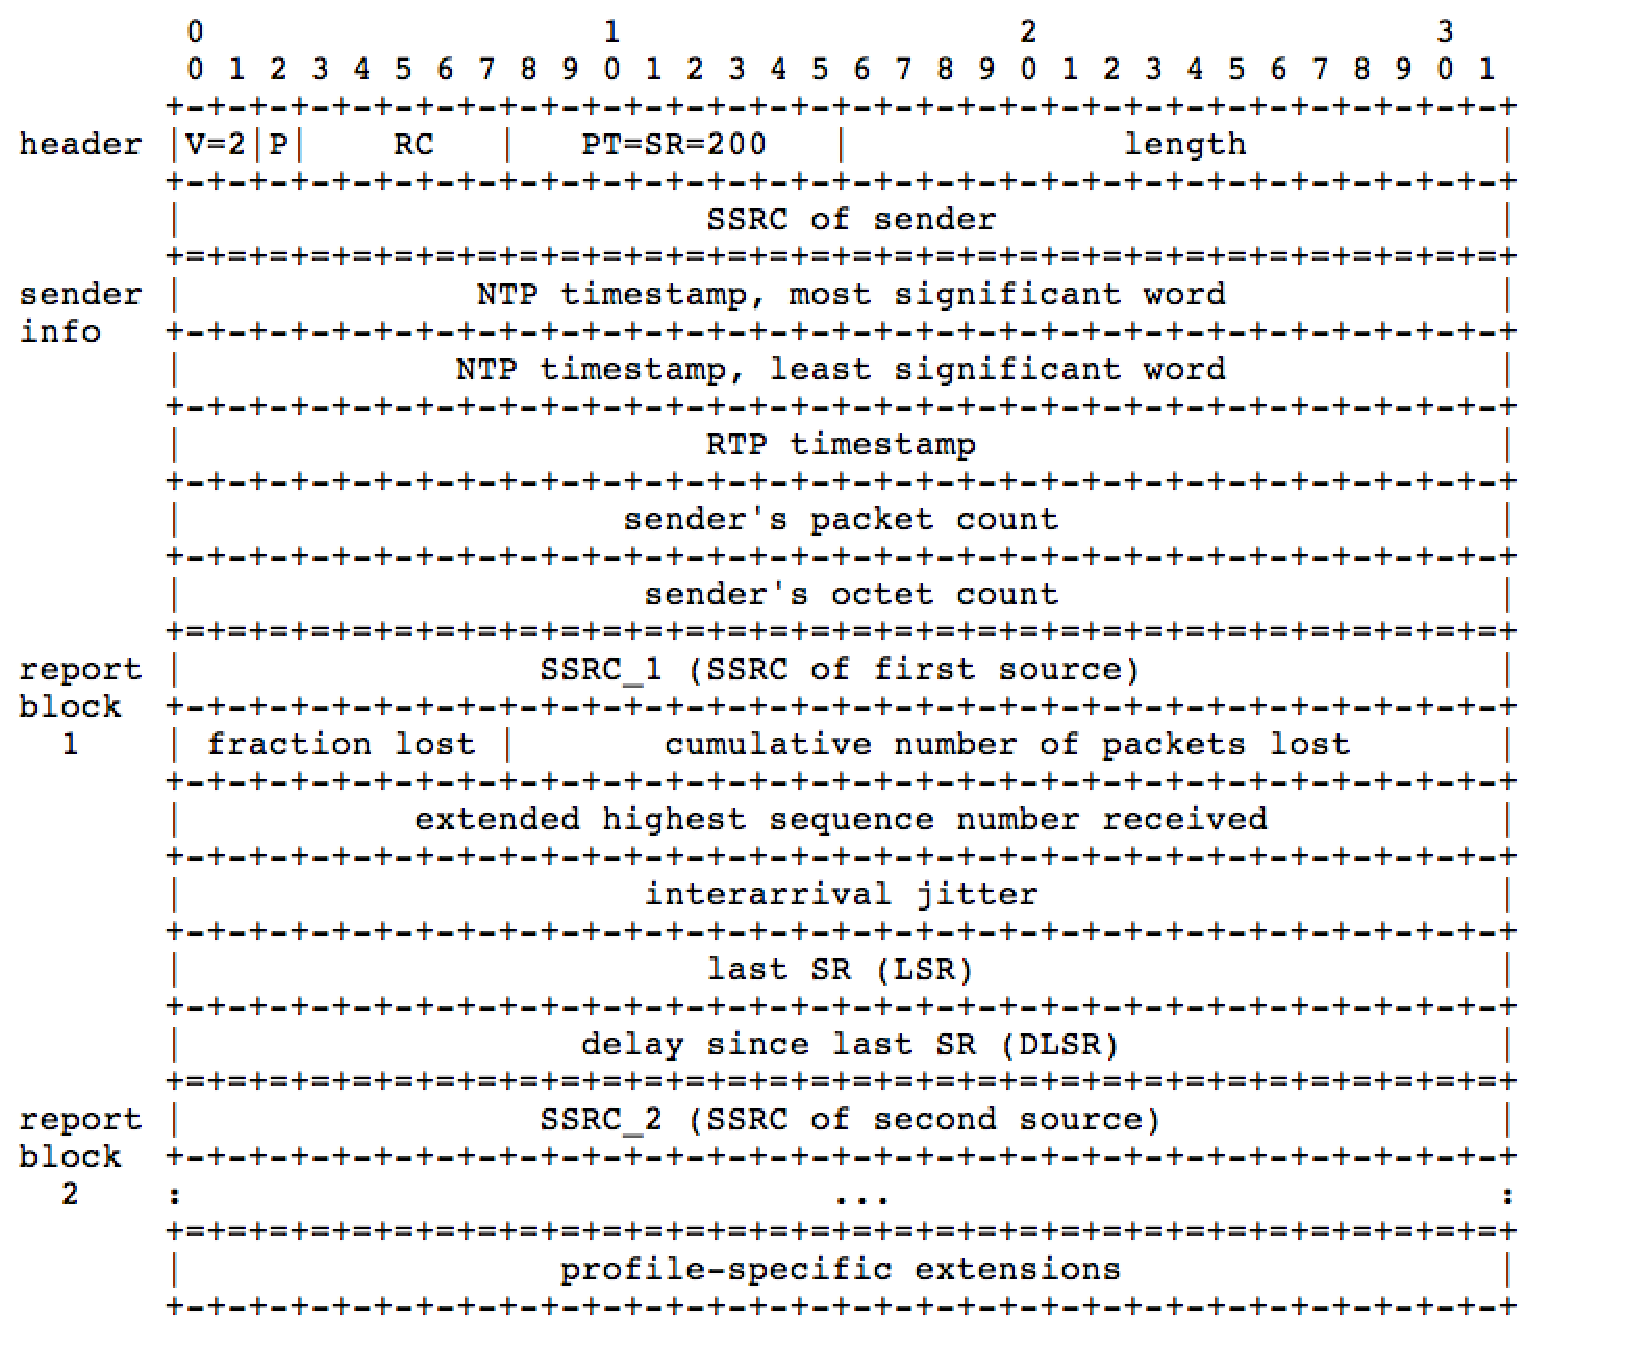
\includegraphics[width=\textwidth]{chap3_fig_hdr_rtcp}}
% \caption{shows the RTCP packet format for carrying the Sender Report (SR) and
% the Receiver Report (RR). The SR carries transport statistics and enables 
% stream synchronization, while the RR carries the receiver transport 
% characteristics.}
% \label{fig:3:rtcp.hdr}
% \end{figure}

The receiver measures the incoming streams and reports the coarse-grained
transport statistics in an RTCP Receiver Report (RR). The RTCP RR contains the
current loss fraction, jitter, highest sequence number received, and
facilitates in calculating the RTT. The sender uses RTCP Sender Reports (SRs)
to assist in synchronizing the media streams (audio and video) by relating the
RTP timestamps of the individual media streams to the wall clock time (NTP)
and to notify the receiver about the current packet rate and bit rate.
Figure~\ref{fig:3:rtcp.hdr} shows the RTCP packet header format for a
interactive unicast media stream (i.e., both sending and receiving media).

\section{RTP Payload Formats}

The general principle for defining payload formats/types is to be able to
identify the encoding of the media packets. These encodings are either  
codec-specific (e.g., H.264, H.263, H.261, MPEG-2, JPEG, G.711, G.722, AMR, etc.),
or generic (e.g., Forward Error Correction (FEC), NACK, multiplexed streams).
Typically a payload document specifies a well-defined packet format for media
codecs; it also defines \emph{aggregation rules} for codecs that produce
several small frames (e.g., audio) compared to the IP Maximum Transmission
Unit (MTU) and \emph{fragmentation rules} for codecs that produce large frames
(e.g., I-frames by video codecs). The main reason to provide fragment large
frames  into smaller packets and not rely on IP fragmentation is, IP
fragmented packets are commonly discarded in the network, especially by NATs
or Firewalls.

% Usually the RTP header is immediately followed by
% payload-specific header (payload format) and then by the media data. This
% allows the sending endpoint to semantically fragment large packets, which
% simplifies processing and decoding at the receiver (i.e., be able to decode
% individual packets without relying on receiving other packets).

\begin{figure}[!h]
\begin{spacing}{0.5}
{\footnotesize
\begin{verbatim}
    0                   1                   2                   3
    0 1 2 3 4 5 6 7 8 9 0 1 2 3 4 5 6 7 8 9 0 1 2 3 4 5 6 7 8 9 0 1
   +-+-+-+-+-+-+-+-+-+-+-+-+-+-+-+-+-+-+-+-+-+-+-+-+-+-+-+-+-+-+-+-+
   |V=2|P|X|  CC   |M|     PT      |       sequence number         |
   +-+-+-+-+-+-+-+-+-+-+-+-+-+-+-+-+-+-+-+-+-+-+-+-+-+-+-+-+-+-+-+-+
   |                           timestamp                           |
   +-+-+-+-+-+-+-+-+-+-+-+-+-+-+-+-+-+-+-+-+-+-+-+-+-+-+-+-+-+-+-+-+
   |           synchronization source (SSRC) identifier            |
   +=+=+=+=+=+=+=+=+=+=+=+=+=+=+=+=+=+=+=+=+=+=+=+=+=+=+=+=+=+=+=+=+
   |                        Payload Format                         |
   +               +-+-+-+-+-+-+-+-+-+-+-+-+-+-+-+-+-+-+-+-+-+-+-+-+
   |               |                                               |
   +-+-+-+-+-+-+-+-+                                               +
   |                           Media Data                          |
   +                                                               +
   |                                                               |
   +-+-+-+-+-+-+-+-+-+-+-+-+-+-+-+-+-+-+-+-+-+-+-+-+-+-+-+-+-+-+-+-+
\end{verbatim}
}
\end{spacing}
\caption{shows the packet structure of an RTP packet encapsulating the
payload-specific header and the associated media data.}
\label{fig:3:pt.fmt}
\end{figure}

% \begin{figure}[!t]
% \centerline{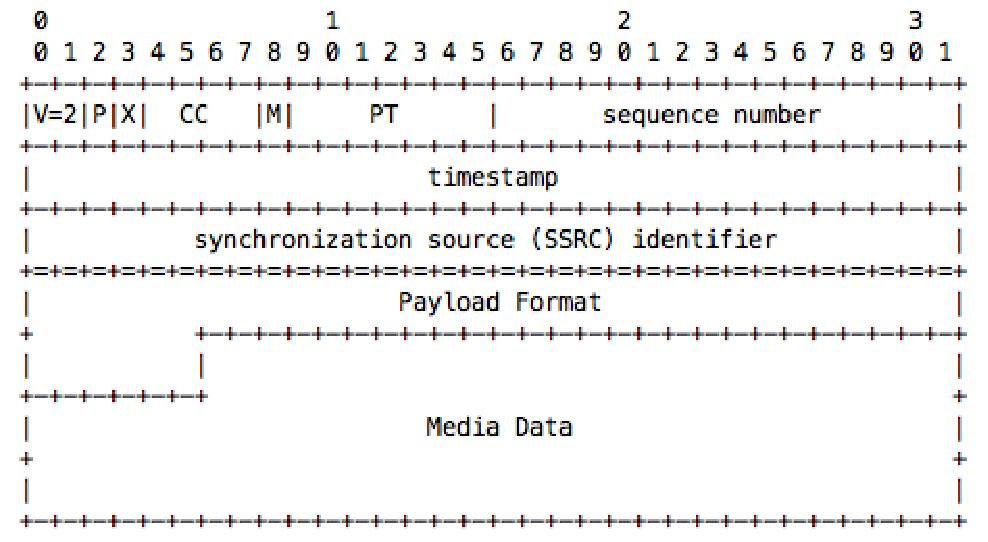
\includegraphics[width=\textwidth]{chap3_fig_hdr_pt_fmt}}
% \caption{shows the packet structure of an RTP packet encapsulating the
% payload-specific header and the associated media data.}
% \label{fig:3:pt.fmt}
% \end{figure}

\section{RTP Header Extensions}

RTP header extensions carry media-independent information, i.e., data that may
be generically applicable to multiple payload formats (e.g., timing
information), and needs to be reported more frequently than RTCP reports are
emitted. A commonly cited example is sending NACKs for interactive video,
where media flows in both directions and RTP packets are generated every tens
of milliseconds, the RTP header extension can indicate which sequence numbers
were correctly received or lost, thereby not completely relying on the RTCP
receiver reports for sending NACKs or ACKs.

The advantage of using header extensions is that they are backwards
compatible, i.e., an endpoint that does not understand them is able ignore
them. Some current use-cases for RTP header extensions are: reporting the
network send timestamp, instead of bursting packets from a large frame on to
the network, the sender paces these packets, client's audio levels (to
equalize audio levels across multiple streams in a video conference).

\section{RTCP Reporting Interval}
% timing

A closed control loop is formed by sending RTP media packets and receiving
RTCP feedback packets. The RTCP feedback interval is typically limited to a
small fraction, so not to affect the media traffic. The RTCP reporting
interval is determined by the number of SSRCs in the session (denoting the
session size), and the chosen session bandwidth. The session bandwidth is
expected to be divided amongst the participants, but oftentimes it is
calculated as the sum of the average throughput of the senders expected to be
concurrently active. In the case of an audio conference the session bandwidth
would be one sender's bandwidth, but for a video conference it would vary
depending on the number of participants displayed on the user interface.
Therefore, the session bandwidth is supplied by the session management
application so that each participants calculates the same value for the RTCP
interval.


The recommended fraction of the session bandwidth allocated for control
traffic is 5\,\%. For many scenarios, including large conferences, where there
are a large number of receivers but a small number of senders, it is
recommended that $\frac{1}{4}^{th}$ of the reporting bandwidth
(\emph{rtcp\_bw}) be shared equally by senders and the rest $\frac{3}{4}^{th}$
by the receivers. The main reason is to allow newly joining participants to
quickly receive the CNAME and synchronization timestamps (from the Sender
Reports) for the sending endpoints. For new participants (even if they are
just receivers) the RTCP interval is halved to quickly declare the presence of
a new participant. Lastly, the recommended value for a fixed minimum RTCP
interval is 5 seconds, while the value for reduced minimum is
$\frac{360}{session\_bw}$.  The fixed minimum RTCP interval of \emph{5\,s} is
suitable for unidirectional links or for sessions that do not require
monitoring the reception quality statistics (e.g., IPTV), while the reduced
minimum RTCP interval is suitable for participants in a unicast bidirectional
multimedia sessions. The reduced minimum RTCP interval is suitable for sending
timely feedback messages to either perform congestion control or error repair,
the interval is shorter than \emph{5\,s} for session bandwidths greater than
\emph{72\,kbps}.

% avpf

If an endpoint detects packet loss or onset of congestion midway through a
reporting interval, the base RTP specification~\cite{rfc3550} (AVP profile)
does not allow sending the RTCP reports early and the endpoint has to wait for
the next scheduled RTCP report. In this case, the slow control loop causes
instability and oscillation in the media bit rate. To overcome this
shortcoming, endpoints implement the Extended RTP Profile for RTCP-Based
Feedback (AVPF profile)~\cite{rfc4585}, an extension to RTP's default timing
rules to enable rapid feedback. This profile allows the endpoint to adjust the
RTCP reporting interval to send the RTCP feedback reports earlier than the
next scheduled RTCP report, sometimes even immediately. As long as reporting
interval on average remains the same. Figure~\ref{fig:3:avpf.interval} shows
that in AVP profile the endpoint reports at regular intervals, whereas in AVPF
it gets the opportunity to send feedback early in every other reporting
interval. Along with the possibility of providing timely feedback, the AVPF
profile also defines a suite of error-resilience feedback messages, namely,
Negative Acknowledgements (NACK), Picture Loss Indication (PLI), Slice Loss
Indication (SLI), Reference Picture Selection Indication (RPSI).

\begin{figure}[!t]
\centering{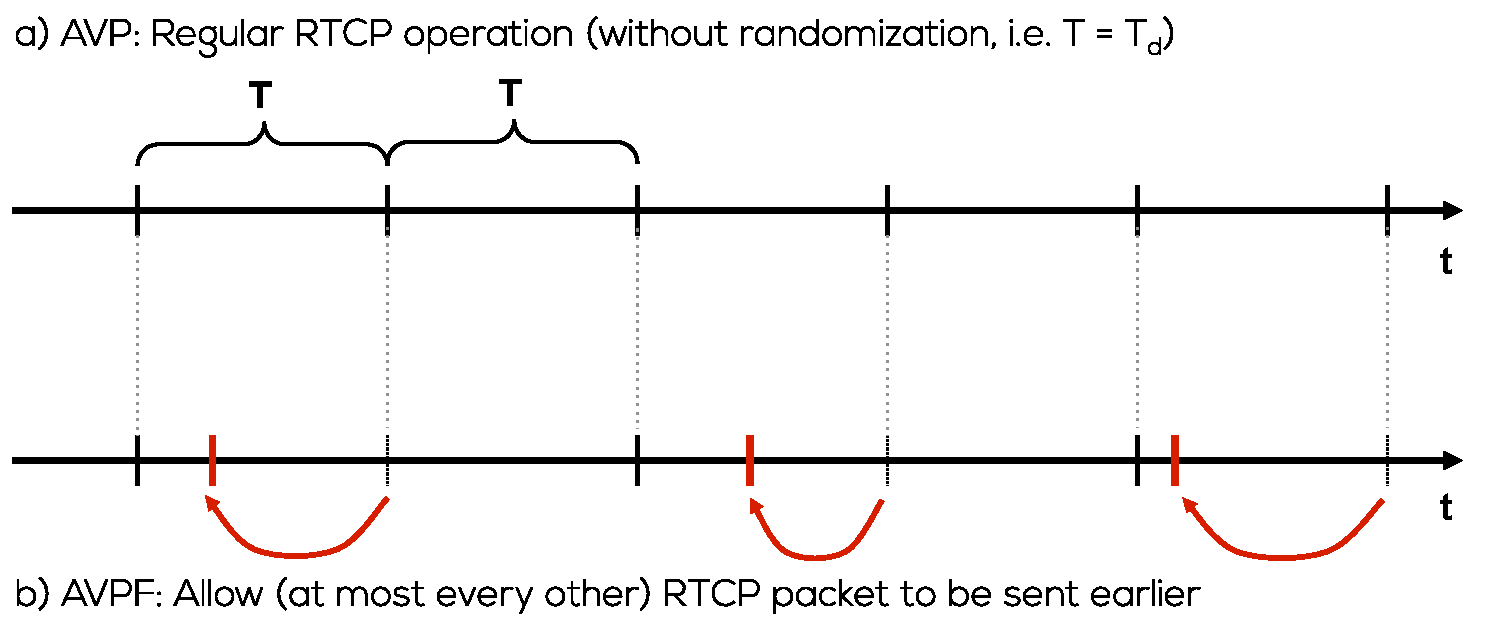
\includegraphics[width=\textwidth]{chap3-fig-avpf-rtcp}}
\caption{shows the RTCP reporting interval as defined in a) AVP, b) AVPF.}
\label{fig:3:avpf.interval}
\end{figure}




\section{RTCP Extended Reports (XRs) for Performance Monitoring}

Endpoints use RTCP Extended Reports (XRs)~\cite{rfc3611} to describe complex
metrics that are not exposed by the RTCP Receiver Report (RR). Some examples of
XRs relevant to performance monitoring and congestion control are: de-jitter
buffer metrics~\cite{rfc7005}, Packet Delay Variation (PDV)~\cite{rfc6798},
delay metric~\cite{rfc6843}, burst-gap discard~\cite{rfc7003}, burst-gap
loss~\cite{rfc6958}, loss Run-Length Encoded (RLE)~\cite{rfc3611}, discard
RLE~\cite{rfc7097}, number of discarded packets~\cite{rfc7002} and
bytes~\cite{draft.xr.bytes.discarded}, summary statistics~\cite{rfc7004},
Quality of Experience (QoE)~\cite{draft.xr.qoe}, and loss
concealment~\cite{draft.xr.conceal}, etc. RTP allows for new metrics to be
defined, the main requirement is to document what is measured, how it is
measured and reported to the other endpoints.


% The RTCP Extended Reports (XR) [RFC3611] allow reporting of more
% complex and sophisticated reception quality metrics, but do not
% change the RTCP timing rules.  RTCP extended reports of potential
% interest for congestion control purposes are the extended packet
% loss, discard, and burst metrics [RFC3611],
% [I-D.ietf-xrblock-rtcp-xr-discard],
% [I-D.ietf-xrblock-rtcp-xr-discard-rle-metrics],
% [I-D.ietf-xrblock-rtcp-xr-burst-gap-discard],
% [I-D.ietf-xrblock-rtcp-xr-burst-gap-loss]; and the extended delay
% metrics [RFC6843], [RFC6798].


\section{Codec Control Messages}
% codec control

Sometimes an endpoint needs to configure or notify the other endpoint's codec.
These messages are broadly classified as \emph{Transport Layer} and \emph
{Payload-specific} feedback messages~\cite{rfc4585, rfc5104}. The transport
layer messages are: Temporary Maximum Media Stream Bit Rate Request (TMMBR)
and Temporary Maximum Media Stream Bit Rate Notification (TMMBN). The
receiving endpoint uses the TMMBR message to configure the maximum encoding
bit rate of the media stream, while the sending endpoint uses the TMMBN to
inform the receiver of the updated bit rate. Therefore, transport layer
feedback messages are intended to transmit general purpose feedback messages,
independent of any particular codec or application.

On the other hand, the payload-specific feedback messages carry information
specific to a certain payload type and is acted upon by the codec layer, some
examples of these type of messages are: Full Intra Request (FIR), temporal-
spatial tradeoff, frame rate, frame size, maximum packet size or packet rate,
etc~\cite{draft.avt.cop}.

\section{Reduced-Size RTCP Reports}
% non-compound feedback

An endpoint sends RTCP feedback as a \emph{compound}, or \emph{minimal} RTCP
packet. A \emph{compound RTCP packet} is defined in~\cite{rfc3585}, contains
at least a sender report (SR) or a receiver report (RR) or both, followed by
Source Description (SDES) and any additional XR blocks. A \emph{minimal RTCP
packet} is one that contains a SR and/or RR, and followed by an SDES
containing just the canonical name (CNAME)\footnote{It is the real name
(identifier) used to describe the source, it can be in any form desired by the
user. Of the SDES items (username, email, phone, geo-location, etc.) CNAME is
compulsory to include in every RTCP packet.}. Hence, every compound RTCP
packet is a minimal RTCP packet with additional report blocks.

Including any of the additional SDES items or adding XR blocks makes the
compound RTCP packet very large. On low bit rate links, these large compound
RTCP packets may introduce more delay. Therefore, it may be desirable to
logically fragment the report blocks in a compound RTCP packet and send them
independently. These fragmented report blocks are called \emph {reduced-size
RTCP packet}~\cite{rfc5506}. Unlike compound RTCP packets, to transmit a
reduced-size RTCP packet an endpoint does not need to include the minimal RTCP
report. However, when using reduced-size RTCP packets, minimal packets need to
be sent once in a while, to keep alive the CNAME-SSRC binding.

Reduced-size RTCP reports are beneficial in wireless networks where the packet
loss rate increases with the packet size, i.e., larger sized packets are more
susceptible to be dropped compared to smaller sized packets. Additionally, smaller
packets have shorter serialization time, i.e., the amount of time it takes for
the endpoint to put the data packet on to the link is short.

The main reasons for the application to use the reduced-size RTCP reports are:
1) notify the other endpoint of events, using the signaling channel would
incur at least one RTT while implementing it as an RTCP extension would merely
incur a one-way delay. 2) send codec control (e.g., TMMBR) or feedback (e.g.,
NACK, RPSI) messages, these messages as reduced-size are more likely to be
transmitted compared to the compound packets and with as little delay as
possible. Especially since these types of messages are more likely to be sent
when link conditions are poor.


% relationship with SDP
\section{Session Setup}

% SDP O/A, declarative SDP, RTCP notify

There are several ways to setup an interactive or conversational multimedia
session, for example by implementing one of the following: H.323~\cite{H.323},
Session Initiation Protocol (SIP)~\cite{rfc3261}, Jingle~\cite{XEP-0166} an
extension to the Extensible Messaging and Presence Protocol
(XMPP)~\cite{rfc6120}.

SIP uses the Session Description Protocol (SDP)~\cite{rfc4566} to describe the
endpoint's transport and media capabilities. An SDP description defines a
single multimedia session, i.e., an association between a set of participants.
It may however, carry multiple media streams in the session.

\begin{figure}[!h]
\centerline{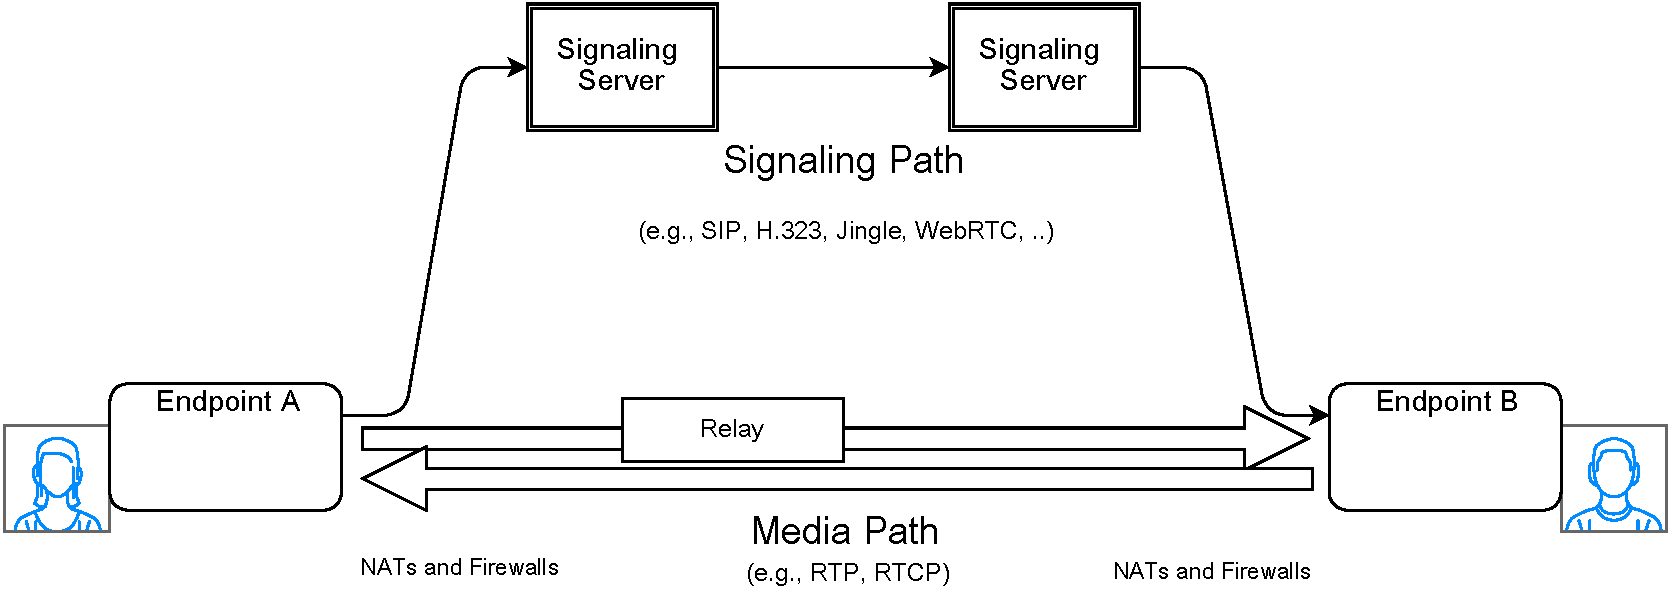
\includegraphics[width=\textwidth]{chap3-fig-sig-med}}
\caption{shows the signaling and media paths between two endpoints engaging in
a video call.}
\label{fig:3:sig.media}
\end{figure}


The transport details in the SDP are mainly split into two parts: the protocol
for delivering media packets (currently, TCP, UDP, or SCTP) and the outgoing
IP address of the endpoint. The protocol to deliver the media packets is
chosen by the application, but identifying the outgoing IP address of an
endpoint is a bit complex and first requires gathering the endpoint's multiple
IP addresses and later exchanging them with the other endpoints to establish
connectivity.

Multiple IP addresses arise not only from multiple interfaces but also due to
the presence of NAT devices in the network, which may change the IP address of
the outgoing packets. Since, interactive media calls are between endpoints and
media streams may eventually traverse through a NAT at both ends, in some
cases, the only way to deliver media packets between the two endpoints would
be by using a relay\footnote{Traversal Using Relays around NAT (TURN)} on the
public Internet. Hence, the endpoint needs to discover its 2-tuple \texttt{[IP
address:port]} on the host, the public address if behind a NAT~\cite{rfc5389}
and the address allocated by the TURN relay~\cite{rfc5766} before it notifies
the other endpoints about its transport details. This collection of 2-tuples
is known as \emph{candidates}, at first the endpoints sort the candidates in
the decreasing order of the candidate's priority and later exchange their
candidate addresses in the SDP with the other endpoint. On receiving the
candidates, the endpoint performs a probe between each combination of
addresses in the two candidate lists and chooses the first one that is
successfully received (\emph{aggressive nomination}). This process of
performing pair-wise \emph{connectivity checks} is called Interactive
Connectivity Establishment (ICE)~\cite{rfc5245, rfc6544} and it relies on
\emph{Session Traversal Utilities for NAT} (STUN) protocol~\cite{rfc5389} to
establish connectivity across a NAT and in case it fails to establish
connectivity, it uses \emph{Traversal Using Relays around NAT} (TURN)
protocol~\cite{rfc5766} to use a relay on the public Internet to deliver the
media packets.

% Depending on the type of NAT device (full-cone, address- or port-restricted
% cone, symmetric).

\begin{figure}[!h]
{\small
\begin{verbatim}
        v=0
        o=jdoe 2890844526 2890842807 IN IP4 10.0.1.1
        s=
        c=IN IP4 192.0.2.3
        t=0 0
        a=ice-pwd:asd88fgpdd777uzjYhagZg
        a=ice-ufrag:8hhY
        m=audio 45664 RTP/AVP 0
        a=rtpmap:0 PCMU/8000
        a=candidate:1 1 UDP 2130706431 10.0.1.1 8998 typ host
        a=candidate:2 1 UDP 1694498815 195.148.127.98 45664 typ srflx 
            raddr 10.0.1.1 rport 8998
\end{verbatim}
}
\caption{Sample SDP containing the sender's transport and media capabilities.}
\label{fig:3:sdp}
\end{figure}

The second part of SDP carries the media capabilities, together with the
transport parameters binds the SDP to the Offer/Answer (O/A) model. In the O/A
model, the sending endpoint \emph{offers} to the receiver a set of media
capabilities in decreasing order of preference, typically, multiple options of
audio/video codecs and ICE candidates. On receiving the sender's capabilities,
the receiver compares its media capabilities with the sender's and responds
with the one that best fits the receiver's requirements (\emph{answer}). The
\emph{offer is rejected} in the case where the receiver is unable to pick any
of the options provided by the sender or if ICE connectivity checks fail.
Hence, the application at the sender needs to pick a minimum number of widely
available audio and video codecs to avoid negotiation failure. If the
\emph{offer is accepted}, both endpoints then know the following: 1) which
audio and/or video codecs to use, 2) the payload types of the encoded media
streams (possibly even their respective SSRCs), 3) to which IP address and
port number to send the media stream, 4) the media session bandwidth, if
indicated and 5) the encryption keys, if encrypting traffic.

\begin{figure}
\centering{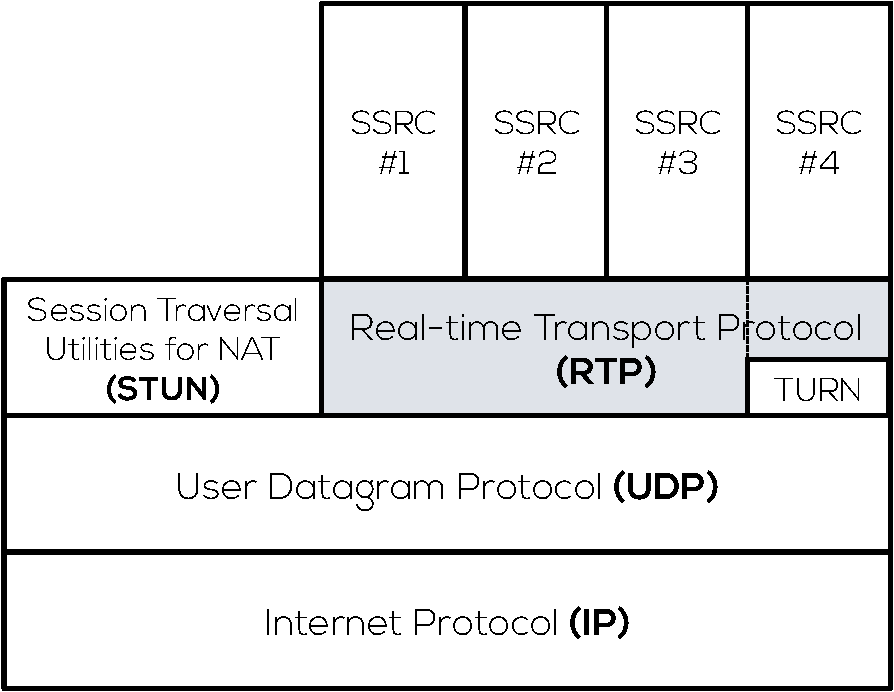
\includegraphics[width=0.9\textwidth]{chap3-fig-rtp-stack}}
\caption{Relationship of RTP with STUN, TURN, DTLS and the signaling protocol.}
\label{fig:3:rtp-stack}
\end{figure}

Figure~\ref{fig:3:rtp-stack} shows the relationship of the RTP stack with the
rest of the IP stack. RTP is usually transmitted over UDP, but under some
constrained situations (e.g., restrictive firewalls or NATs) it may be
encapsulated in TCP~\cite{rfc3550}. STUN~\cite{rfc5389} is used by ICE to
discover the presence of a NAT device and obtain the mapped (public) IP
address. When using a TURN relay server (in the presence of symmetric NATs or
not to reveal the host address of the caller for privacy reasons), the RTP
packets are encapsulated inside the TURN's \texttt{ChannelData}
message~\cite{rfc5766}. In the Figure~\ref{fig:3:rtp-stack} four media streams
(SSRC \#1-4) are transmitted by RTP over UDP, but two streams (SSRC \#1-2) are
relayed through a TURN server. Secure RTP (SRTP)~\cite{rfc3611} is a security
framework that provides confidentiality by encrypting RTP payload (not the RTP
headers) and supports source origin authentication. While SRTP is not the only
security mechanism for RTP~\cite{draft.srtp-not-must}, it is widely
applicable, especially to voice telephony and group communication. However,
the main challenge for SRTP is key management~\cite{draft.sec-opts}, here too
many options exist (e.g., SRTP over DTLS in WebRTC~\cite{rfc5763}, MIKEY in
SIP~\cite{rfc3830}, Security Description in SDP~\cite{rfc4566},
ZRTP~\cite{RFC6189}, etc.).

\section{Summary}

In this chapter we introduce the protocol features of RTP and RTCP, the
mechanisms to extend it, including numerous profiles and feedback reports. We
also discuss the limitations to RTCP reporting interval and the reliance on
signaling for setting up the media session between endpoints.

